\chapter{Marco Metodológico: Arquitectura General del Sistema}

Los algoritmos actuales de reconstrucción, como Multi View Stereo (MVS), operan bajo un paradigma de densificación exhaustiva. El problema principal de este enfoque es que resulta excesivamente costoso y redundante computacionalmente, ya que intenta densificar millones de píxeles sin entender la estructura de lo que está reconstruyendo. Generar estas nubes masivas se vuelve inmanejable para entornos urbanos a gran escala.

Para solucionar esto, el sistema propuesto plantea un modelo basado firmemente en la abstracción semántica y geométrica. En lugar de procesar a ciegas la profundidad, el enfoque busca comprender primero la escena arquitectónica para luego triangular únicamente las primitivas estructurales necesarias. 

Este capítulo presenta un resumen rápido y estructurado de las fases que conforman la arquitectura propuesta, delineando la idea general del proyecto. Los detalles matemáticos y la implementación técnica profunda de cada fase se abordarán con muchísimo detalle en los capítulos posteriores.

\section{Pipeline de Reconstrucción}
El \textit{pipeline} propuesto abandona por completo la densificación clásica basada en píxeles. Esto funciona dividiendo el problema en fases secuenciales, priorizando en todo momento la extracción de caras y fronteras arquitectónicas. El flujo de datos y los modelos involucrados en cada etapa se ilustran en la Figura \ref{fig:pipeline_general}.

\begin{figure}[H]
    \centering
    \resizebox{0.95\textwidth}{!}{
    \begin{tikzpicture}[
        node distance=0.8cm and 0.5cm,
        phase/.style={rectangle, draw=blue!60, fill=blue!5, very thick, minimum width=4cm, minimum height=1.2cm, text centered, rounded corners, font=\small\bfseries, align=center},
        input/.style={rectangle, draw=gray!60, fill=gray!5, very thick, minimum width=3.5cm, minimum height=1cm, text centered, font=\footnotesize, align=center},
        arrow/.style={thick, -Latex, draw=black!70}
    ]

    % Nodes
    \node (video) [input] {Video Original (RGB)};
    
    \node (fase1) [phase, below=of video] {Fase 1: Preprocesamiento \\ (Enmascaramiento)};
    \node (vidmask) [input, below=of fase1] {Video Enmascarado};
    
    \node (fase2) [phase, below left=1cm and 0.1cm of vidmask] {Fase 2: Extracción y Tracking \\ (Co-PLNet + GlueStick)};
    \node (fase3) [phase, below right=1cm and 0.1cm of vidmask] {Fase 3: Segmentación de Caras \\ (SAM / ZeroPlane)};
    
    \node (poses) [input, below=of fase2] {Poses de Cámara \\ \& Wireframes 2D};
    \node (masks) [input, below=of fase3] {Máscaras Planares \\ Semánticas};
    
    \node (fase4) [phase, below=4.5cm of vidmask] {Fase 4: Fusión Temporal y Completado \\ (LO-RANSAC)};
    \node (planos) [input, below=of fase4] {Planos Infinitos 3D};
    
    \node (fase5) [phase, below=of planos] {Fase 5: Extracción de Fronteras \\ y Texturizado (Homografías)};
    \node (output) [input, below=of fase5] {Modelo 3D Estructurado \\ (Malla Poligonal)};

    % Arrows
    \draw [arrow] (video) -- (fase1);
    \draw [arrow] (fase1) -- (vidmask);
    
    \draw [arrow] (vidmask) -| (fase2);
    \draw [arrow] (vidmask) -| (fase3);
    
    \draw [arrow] (fase2) -- (poses);
    \draw [arrow] (fase3) -- (masks);
    
    \draw [arrow] (poses) |- (fase4);
    \draw [arrow] (masks) |- (fase4);
    
    \draw [arrow] (fase4) -- (planos);
    \draw [arrow] (planos) -- (fase5);
    \draw [arrow] (fase5) -- (output);
    
    % Feedback
    \draw [arrow, dashed] (poses.west) -- +(-1.5,0) |- (fase5.west) node[pos=0.25, left, font=\scriptsize] {Líneas proyectadas};

    \end{tikzpicture}
    }
    \caption[Diagrama de flujo del pipeline propuesto]{Diagrama de flujo del pipeline de reconstrucción \textit{top-down}. Se detallan las entradas, fases de procesamiento y salidas para la obtención de mallas poligonales limpias.}
    \label{fig:pipeline_general}
\end{figure}

\subsection{Fase 1: Preprocesamiento y Enmascaramiento Dinámico}
Esta fase sirve para limpiar las secuencias de video de información no deseada. Funciona a través de modelos de inferencia rápida, como FastSAM o YOLO, los cuales detectan objetos dinámicos dentro de la escena (típicamente autos y peatones), tal como se ejemplifica en la Figura \ref{fig:yolo_masking}.

\begin{figure}[H]
    \centering
    \begin{minipage}{0.48\textwidth}
        \centering
        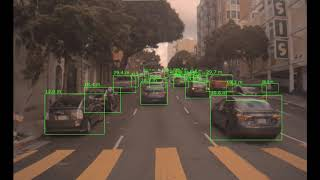
\includegraphics[width=\linewidth]{images/yolo_masking.png}
    \end{minipage}\hfill
    \begin{minipage}{0.48\textwidth}
        \centering
        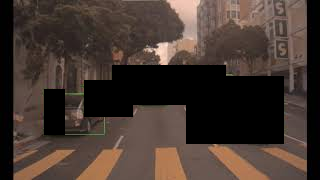
\includegraphics[width=\linewidth]{images/yolo_blacked.png}
    \end{minipage}
    \caption{Proceso de preprocesamiento: Identificación de elementos dinámicos con YOLO (izquierda) y su posterior enmascaramiento o censura espacial (derecha) para evitar ruido en la geometría (Fuente: Adaptado de \url{https://youtu.be/ftsUg5VlzIE}).}
    \label{fig:yolo_masking}
\end{figure}

Una vez identificados, se aplica un enmascaramiento dinámico (\textit{Masking}) para omitir estas regiones temporalmente de los cálculos geométricos. Un enfoque alternativo que muchos podrían sugerir es rellenar estos vacíos utilizando técnicas de \textit{Video Inpainting} previo a la reconstrucción. Sin embargo, como lo advierte la literatura en sistemas de mapeo dinámico \cite{bescos2018dynaslam}, la desventaja crítica del \textit{inpainting} generativo no es su tiempo de cómputo, sino su \textbf{inestabilidad geométrica}. 

Estos modelos \textit{alucinan} texturas visualmente plausibles pero carentes de consistencia temporal. Esta inestabilidad genera parpadeos y características falsas entre \textit{frames} que terminan corrompiendo de forma irremediable la geometría epipolar y el rastreo (\textit{tracking}) de la cámara.

\begin{itemize}
    \item \textbf{Resumen:} Se usan modelos de segmentación rápida para enmascarar y descartar los objetos móviles, optando por ignorar la información en lugar de inventarla con \textit{inpainting}, salvaguardando así la pureza matemática del sistema.
\end{itemize}

\subsection{Fase 2: Extracción Estructural y Tracking Híbrido}
El objetivo de esta fase es rastrear la trayectoria de la cámara y obtener la estructura base evadiendo los descriptores clásicos basados en texturas, como SIFT o ORB, porque son propensos a fallar en entornos repetitivos o sin textura. 

Se utilizan arquitecturas neuronales de última generación, como Co-PLNet \cite{wang2026coplnet}, para extraer nodos clave y los \textit{wireframes} estructurales en cada imagen. Como se observa en la Figura \ref{fig:coplnet_examples}, la red identifica con precisión las esquinas y líneas arquitectónicas de la edificación. 

\begin{figure}[H]
    \centering
    \begin{minipage}{0.48\textwidth}
        \centering
        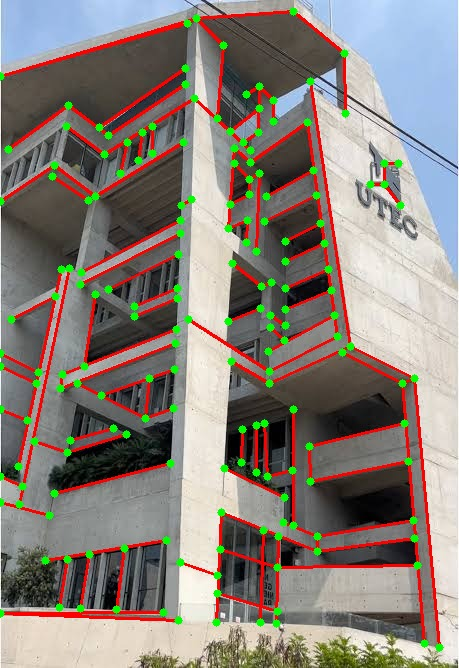
\includegraphics[width=\linewidth]{images/coplnet_utec1.png}
    \end{minipage}\hfill
    \begin{minipage}{0.48\textwidth}
        \centering
        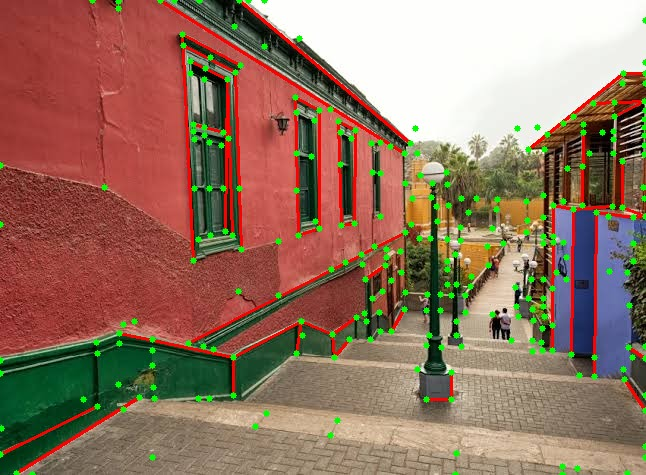
\includegraphics[width=\linewidth]{images/coplnet_barranco.png}
    \end{minipage}
    \caption{Demostración de extracción conjunta de puntos y líneas sobre edificaciones reales utilizando Co-PLNet. Se observan los nodos estructurales en verde y las fronteras arquitectónicas en rojo (Fuente: Elaboración propia).}
    \label{fig:coplnet_examples}
\end{figure}

Posteriormente, se aplican arquitecturas GNN especializadas, específicamente GlueStick \cite{pelaez2023gluestick}, para realizar un emparejamiento inyectivo robusto de puntos y líneas a través del algoritmo de asignación convexa de Sinkhorn. Naturalmente, el costo asintótico original del operador de atención cruzada de Sinkhorn escala a $\mathcal{O}(V^2)$, donde $V$ es la suma de primitivas (líneas y puntos). Para prevenir una explosión paramétrica en la memoria VRAM durante el modelado metropolitano, el pipeline adopta heurísticas de localidad (\textit{Pruning} espacial) en la capa de atención. Esta restricción explota el particionamiento conexo de las geometrías cercanas para inducir una matriz de afinidad rala (\textit{Sparse Affinity Matrix}), suprimiendo la conectividad entre nodos estructurales distantes. Esto permite computar de forma eficiente la triangulación geométrica y recuperar de manera estable el \textit{tracking} de cámara $\mathbf{T} \in SE(3)$.

\subsection{Fase 3: Segmentación y Detección de Caras (Planos)}
En esta etapa, el sistema inyecta restricciones semánticas para detectar y segmentar los planos arquitectónicos dominantes usando modelos especializados como ZeroPlane \cite{liu2025zeroplane}, PlaneRCNN \cite{liu2019planercnn}, o combinaciones robustas usando DUSt3R \cite{wang2024dust3r} y SAM. Como se ejemplifica en la Figura \ref{fig:plane_segmentation}, estas arquitecturas son capaces de identificar y aislar matemáticamente las distintas instancias planas que componen la escena.

\begin{figure}[H]
    \centering
    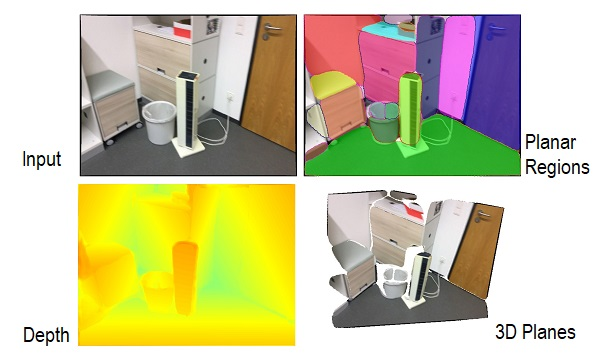
\includegraphics[width=0.95\textwidth]{images/planercnn_segmentation.jpg}
    \caption[Demostración de segmentación de superficies planares]{Demostración de segmentación de superficies planares. La imagen ilustra cómo la red infiere máscaras para cada instancia plana detectada. Cada color representa un plano geométrico distinto, facilitando la distinción entre superficies arquitectónicas y elementos ajenos (Fuente: \cite{liu2019planercnn}).}
    \label{fig:plane_segmentation}
\end{figure}

Analíticamente, la segmentación de planos proporciona restricciones geométricas severas para la reconstrucción. Como se aprecia en la Figura \ref{fig:plane_segmentation}, al asignar a cada píxel su pertenencia a una instancia plana específica, el sistema discrimina las superficies puramente arquitectónicas (fachadas, calzadas, muros) de las geometrías de alta entropía (como vegetación o mobiliario urbano). Esta clasificación semántica permite que las geometrías complejas sean excluidas de la optimización del plano infinito, encapsulándolas temporalmente en volúmenes delimitadores (\textit{bounding boxes}) para evitar que su topología irregular corrompa la instanciación matemática de las caras principales.

\begin{itemize}
    \item \textbf{Resumen:} Se aíslan las caras planares útiles de las geometrías complejas garantizando que solo la estructura puramente arquitectónica guíe la reconstrucción 3D.
\end{itemize}

\subsection{Fase 4: Fusión Temporal, Tracking Semántico y Completado Geométrico}
El reto algorítmico en este punto es lograr mallas continuas manteniendo la coherencia espacial a través del flujo de video sin acoplamiento temporal excesivo. Esto se resuelve estructurando un \textbf{Grafo de Seguimiento de Instancias (\textit{Instance Tracking Graph})} para fusionar temporalmente las caras segmentadas. Esta estructura de datos bidimensional rastrea la identidad topológica de los "super-segmentos" en tiempo de ejecución, propagando sus ID a través de \textit{bounding boxes} superpuestas entre fotogramas consecutivos con una complejidad de actualización asintótica acotada a $\mathcal{O}(I \log I)$ mediante árboles de particionamiento, siendo $I$ el número de instancias activas.

Sobre este grafo cohesivo de segmentos fusionados, el sistema recupera los puntos estructurales conocidos provenientes del \textit{wireframe} (Fase 2). Para la instanciación paramétrica del plano subyacente $\boldsymbol{\pi}$, se emplea el algoritmo \textit{Locally-Optimized RANSAC} (LO-RANSAC) \cite{lebeda2012loransac}. Sin embargo, LO-RANSAC no se utiliza como un mero clasificador, sino como un optimizador estocástico riguroso. Su objetivo es hallar los coeficientes del plano 3D que minimicen la Función de Coste del Error de Reproyección Geométrico $\mathcal{L}_{\text{geom}}$ en las $M$ vistas donde el plano es co-visible:
\begin{equation}
    \boldsymbol{\pi}^* = \arg\min_{\boldsymbol{\pi}} \sum_{m=1}^{M} \sum_{\mathbf{x} \in \mathcal{S}_m} \rho \left( \left\| \mathbf{x} - f_m(\mathbf{P} \mathbf{X}(\mathbf{x}, \boldsymbol{\pi})) \right\|_\Sigma \right)
\end{equation}
Donde $\mathbf{x}$ son los nodos estructurales 2D, $\mathbf{P}$ es la matriz de cámara, y $\mathbf{X}$ es el rayo invertido intersecando el plano de hipótesis $\boldsymbol{\pi}$. La función $\rho(\cdot)$ es un estimador robusto (e.g., coste de Huber) que mitiga la contribución escalar de \textit{outliers} geométricos. La resolución de este coste no lineal garantiza que los vértices arquitectónicos sean retro-proyectados minimizando el error epipolar, garantizando así una instanciación algebraicamente estricta de los muros.

\subsection{Fase 5: Extracción de Fronteras, Reconciliación Topológica y Texturizado}
RANSAC devuelve una abstracción matemática infinita. Esta fase sirve para delimitar físicamente esa superficie utilizando las líneas proyectadas del \textit{wireframe} (Fase 2) para recortar el plano infinito, estableciendo las fronteras reales del polígono arquitectónico.

Sin embargo, como lo exige la geometría algorítmica, proyectar polígonos independientes genera topológicamente una "sopa de polígonos" (\textit{polygon soup}). Para evitar fallas críticas como intersecciones en T (\textit{T-junctions}) o modelos no estancos (\textit{non-watertight}) llenos de huecos, el sistema aplica un post-procesamiento de \textbf{Reconciliación Topológica}. Matemáticamente, se detectan los planos cuyas normales son altamente ortogonales (esquinas de un edificio) o colineales, y se intersectan espacialmente en $\mathbb{R}^3$ para fusionar ("coser") sus vértices frontera. Este ensamble algorítmico garantiza que la malla extraída preserve las invariantes topológicas de una variedad bidimensional (\textit{2-manifold surface}).

Una vez instanciado este polígono 3D cerrado y estanco, se le aplica el texturizado. Para garantizar un mapeo UV de alta fidelidad, se proyecta la textura desde el fotograma cuya pose posea el eje óptico más colineal con la normal de la superficie (es decir, maximizando el producto escalar $\mathbf{n} \cdot \mathbf{v}_{\text{cam}}$). 

El mapeo de textura no es un simple \textit{warp} 2D, sino una homografía inducida analíticamente por la geometría en $SE(3)$. Dado el plano infinito parametrizado como $\boldsymbol{\pi} = (\mathbf{n}^T, d)^T$, la matriz homográfica $\mathbf{H}$ que transfiere los píxeles de la cámara de textura hacia el plano estructural se deriva de la métrica proyectiva canónica:
\begin{equation}
    \mathbf{H} = \mathbf{K} \left( \mathbf{R} - \frac{\mathbf{t} \mathbf{n}^T}{d} \right) \mathbf{K}^{-1}
\end{equation}
Donde $\mathbf{R}$ y $\mathbf{t}$ corresponden a la rotación y traslación relativa entre la vista elegida y el sistema coordenado global del plano, permitiendo una extracción fotométrica algebraicamente exacta, exenta de distorsiones de perspectiva oblicua.

\section{Infraestructura de la Base de Datos de Poses y Alineación Topológica}
La captura asíncrona de datos urbanos a gran escala genera múltiples secuencias de video independientes, las cuales resultan en sub-mapas locales o trayectorias de cámara inconexas. El paradigma clásico comete el error de almacenar nubes de puntos densas directamente en una base de datos. Sin embargo, en esta propuesta arquitectónica \textbf{se prioriza almacenar el grafo de poses de la cámara en lugar de la geometría cruda}.

Esta decisión de diseño es crítica. Al guardar únicamente las transformaciones espaciales optimizadas ($SE(3)$) y las imágenes fuente, el sistema funciona como un "esqueleto" que es independiente del motor de renderizado. Como se ilustra en la Figura \ref{fig:pose_database}, esto garantiza que el \textit{dataset} recolectado sea completamente agnóstico y reutilizable a futuro. Mañana más tarde, el mismo grafo espacial podrá alimentar no solo la reconstrucción de mallas poligonales actual, sino algoritmos de \textit{3D Gaussian Splatting}, representaciones neuronales (NeRF) o sistemas de mapas interactivos y realidad aumentada.

\begin{figure}[H]
    \centering
    \resizebox{0.95\textwidth}{!}{
    \begin{tikzpicture}[
        node distance=1cm and 1.5cm,
        source/.style={rectangle, draw=red!60, fill=red!5, very thick, minimum width=3cm, minimum height=1cm, text centered, rounded corners, font=\small, align=center},
        db/.style={cylinder, draw=black!70, fill=yellow!10, very thick, minimum width=3.5cm, minimum height=3cm, text centered, aspect=0.3, shape border rotate=90, font=\small\bfseries, align=center},
        app/.style={rectangle, draw=green!60, fill=green!5, very thick, minimum width=4cm, minimum height=1cm, text centered, rounded corners, font=\small, align=center},
        arrow/.style={thick, -Latex, draw=black!70}
    ]

    % Sources
    \node (vid1) [source] {Secuencias de Video};
    \node (gps) [source, below=1cm of vid1] {Telemetría GPS};
    
    % DB
    \node (db) [db, right=2.5cm of vid1, yshift=-0.5cm] {Base de Datos \\ de Poses $SE(3)$ \\ \textit{(Cero nubes densas)}};
    
    % Applications
    \node (app2) [app, right=2.5cm of db, yshift=1.5cm] {3D Gaussian Splatting};
    \node (app1) [app, above=0.5cm of app2] {Mallas Poligonales \\ \textit{(Pipeline Actual)}};
    \node (app3) [app, below=0.5cm of app2] {Campos Radiantes (NeRF)};
    \node (app4) [app, below=0.5cm of app3] {Mapas 3D Interactivos};

    % Arrows
    \draw [arrow] (vid1) -- (db.140);
    \draw [arrow] (gps) -- (db.220) node[midway, below, font=\scriptsize, align=center] {Anclaje y \\ Restricciones};
    
    \draw [arrow] (db.east) -- +(0.8,0) |- (app1.west);
    \draw [arrow] (db.east) -- +(0.8,0) |- (app2.west);
    \draw [arrow] (db.east) -- +(0.8,0) |- (app3.west);
    \draw [arrow] (db.east) -- +(0.8,0) |- (app4.west);

    \end{tikzpicture}
    }
    \caption[Diagrama de la Infraestructura de Poses]{Arquitectura de la Base de Datos de Poses. Al almacenar y alinear el grafo espacial en lugar de puntos tridimensionales masivos, el sistema actúa como un núcleo topológico versátil que puede alimentar múltiples tecnologías de reconstrucción a futuro.}
    \label{fig:pose_database}
\end{figure}

El desafío fundamental radica en la alineación topológica de estas trayectorias relativas hacia un marco de coordenadas global. A nivel algorítmico, esto exige resolver un problema de Optimización de Grafo de Poses (\textit{Pose Graph Optimization}, PGO). Dado que el grupo de similitud $Sim(3)$ posee 7 grados de libertad, la escala absoluta ($s$) es matemáticamente inobservable en secuencias monoculares puras debido a la ambigüedad de \textit{gauge}. 

Para anclar las trayectorias y resolver $T \in Sim(3)$ entre sub-mapas, el sistema extrae coincidencias empleando el método de Horn (alineamiento de Procrustes) sobre la intersección de vértices estructurales (mínimo 3 puntos no colineales). El PGO formula la fusión global minimizando una función de coste multivariable que integra las odometrías relativas $\mathbf{T}_{ij} \in SE(3)$ con restricciones afines absolutas de la telemetría GPS para mitigar la deriva inercial (\textit{drift}). La función de energía sobre el estado $\mathcal{X} = \{ \mathbf{T}_i \}$ se define axiomáticamente como:
\begin{equation}
    E_{PGO}(\mathcal{X}) = \sum_{(i,j) \in \mathcal{E}} \left\| \log_{SE(3)}\left( \mathbf{T}_{ij}^{-1} (\mathbf{T}_i^{-1} \mathbf{T}_j) \right) \right\|_{\boldsymbol{\Sigma}_{ij}}^2 + \sum_{k \in \mathcal{C}} \left\| \mathbf{t}_k - \mathbf{p}_k^{\text{GPS}} \right\|_{\boldsymbol{\Sigma}_{\text{GPS}}}^2
\end{equation}
Para mitigar la acumulación de error inercial y de escala (\textit{drift}), intrínseco al rastreo monocular en distancias prolongadas, la infraestructura integra datos de telemetría GPS. Estos actúan como restricciones absolutas dentro del grafo de optimización. Para garantizar la \textbf{escalabilidad asintótica} de esta base de datos masiva, el sistema indexa espacialmente las posiciones de las cámaras $\mathbf{t}_i$ mediante una estructura jerárquica de particionamiento espacial bidimensional \textbf{KD-Tree}. Esto permite que las consultas computacionales de vecindad para la detección de cierres de bucle (Loop Closure) eludan la comparación exhaustiva ingenua $\mathcal{O}(N^2)$ a través de un volumen de datos masivo, reduciendo la complejidad de búsqueda y acoplamiento estructural a un costo logarítmico $\mathcal{O}(N \log N)$. Esta arquitectura descentralizada y algorítmicamente escalable garantiza la consistencia global a nivel metropolitano, facultando al sistema a ensamblar continuamente nuevos fragmentos de la ciudad sin la penalidad paramétrica de re-optimizar nubes de puntos densas.

\section{Métricas de Evaluación y Entorno Experimental}
Para evaluar rigurosamente la calidad de la reconstrucción y la eficiencia del modelo propuesto frente al estado del arte, se han definido métricas tanto geométricas como computacionales. Asimismo, se ha seleccionado un entorno de pruebas estandarizado que garantice la reproducibilidad del experimento.

\subsection{Dataset de Evaluación: UrbanScene3D}
Las pruebas cuantitativas se realizarán utilizando \textbf{UrbanScene3D} \cite{shen2021urbanscene3d}, un \textit{dataset} a gran escala y simulador diseñado específicamente para la investigación en reconstrucción 3D y percepción urbana por visión estéreo y drones.

\begin{figure}[H]
    \centering
    
\includegraphics[width=0.85\textwidth]{images/urbanscene3d.jpg}
    \caption[Entorno de simulación y dataset UrbanScene3D]{Representación de una de las ciudades del dataset UrbanScene3D. Provee secuencias de video de alta resolución, parámetros de cámara exactos y un modelo geométrico (\textit{Ground Truth}) extremadamente preciso, lo que resulta fundamental para contrastar matemáticamente la fidelidad de la malla extraída (Fuente: Adaptado de \cite{shen2021urbanscene3d}).}
    \label{fig:urbanscene3d}
\end{figure}

UrbanScene3D fue elegido por encima de otros repositorios porque ofrece secuencias de imágenes aéreas sintéticas y reales junto con un modelo topológico completo. Disponer del \textit{Ground Truth} de la geometría arquitectónica permite evaluar sin margen de error la hipótesis del \textit{pipeline} libre de MVS.

\subsection{Métricas Geométricas}
Estas métricas, extraídas del estándar del estado del arte, miden qué tan parecida es la topología reconstruida ($P$) respecto a la escena de referencia o \textit{Ground Truth} ($G$).

\begin{itemize}
    \item \textbf{RMSE(P, G) - Error Cuadrático Medio Posicional:} Cuantifica la desviación posicional absoluta promedio de los vértices extraídos frente a la malla real. Mide directamente cuánto se equivocó el algoritmo al ubicar la geometría en el espacio euclidiano. Se define como:
    \begin{equation}
        \text{RMSE}(P, G) = \sqrt{\frac{1}{|P|} \sum_{p \in P} \min_{g \in G} \|p - g\|_2^2}
    \end{equation}
    Donde $p$ y $g$ representan puntos homólogos en ambas nubes.

    \item \textbf{$\mathbf{d_{CD}(P, G)}$ - Distancia de Chamfer:} Es la métrica estándar por excelencia para evaluar mallas 3D. Intuitivamente, calcula, para cada punto de la reconstrucción $P$, cuál es su vecino más cercano en la geometría real $G$ (evaluando Precisión), y viceversa desde $G$ hacia $P$ (evaluando Completitud). Se define formalmente como:
    \begin{equation}
        d_{CD}(P, G) = \frac{1}{|P|} \sum_{p \in P} \min_{g \in G} \|p - g\|_2^2 + \frac{1}{|G|} \sum_{g \in G} \min_{p \in P} \|p - g\|_2^2
    \end{equation}
    Un valor cercano a cero penaliza fuertemente las mallas que inventan "geometrías fantasma" (mala precisión) o que dejan huecos estructurales (mala completitud).

    \item \textbf{Error Absoluto Topológico (Normales):} Evalúa la integridad de las caras arquitectónicas y la preservación de los bordes duros de los edificios. En arquitecturas \textit{Manhattan-world}, esto se mide mediante el error angular de las normales de las superficies:
    \begin{equation}
        \text{EAT}(P, G) = \frac{1}{|P|} \sum_{i=1}^{|P|} \arccos(|\mathbf{n}_{P,i} \cdot \mathbf{n}_{G,i}|)
    \end{equation}
    Penaliza severamente el ruido estructural, como las paredes que parecen "derretidas" o con deformaciones, típicas de los enfoques MVS cuando se confunden con reflejos en las ventanas.
\end{itemize}

\subsection{Métricas Computacionales}
Dado que el objetivo principal y la promesa de valor de la investigación es aniquilar el excesivo coste computacional del MVS clásico, se evaluarán dos parámetros operativos críticos de hardware:

\begin{itemize}
    \item \textbf{Tiempo de Cómputo (Horas):} Se cronometrará el tiempo exacto transcurrido desde la ingesta de las imágenes hasta la exportación de la malla poligonal final. El objetivo es comprobar empíricamente una reducción logarítmica en los tiempos de inferencia.
    \item \textbf{Consumo máximo de memoria (Peak VRAM):} Mide la huella de memoria en gigabytes (GB) requerida en la tarjeta gráfica. Con esta métrica se busca demostrar empíricamente que extraer únicamente la abstracción geométrica requiere una fracción marginal de la VRAM comparado con densificar iterativamente millones de píxeles ciegos.
\end{itemize}